\chapter{LTSpice VII: Resumen }\label{LTspice}

\hspace{10pt} LTSpice VII es un software de simulación  de circuitos eléctricos y electrónicos, que partiendo de una captura esquemática, realiza una simulación rápida y de alto rendimiento del circuito en cuestión utilizando modelos eficientes de los componentes involucrados. Este software es distribuido libremente por su fabricante Analog Devices, Inc, pudiéndose descargar de: https://www.analog.com/en/design-center/design-tools-and-calculators/ltspice-simulator.html. El software corre bajo las distintas versiones de Windows.


LTSpice se basa en el software SPICE (Simulation Program with Integrated Circuits Emphasis), desarrollado por por L. Nagel y D. Pederson  en la Universidad de California, Berkeley en 1973, convirtién\-dose en un  estándar internacional para simular circuitos electrónicos analógicos \cite{Nagel75} \cite{queiros91}.

El estándar SPICE realiza tres tipos fundamentales de análisis de circuitos:

\begin{itemize}
    \item Análisis de corriente continua (CC), que obtiene el comportamiento estacionario del circuito
    \item Análisis de corriente alterna (CA), que examina el comportamiento en régimem permanente con onda senoidal.
    \item Análisis transitorio (TRAN), que obtiene  el comportamiento transitorio del circuito
\end{itemize}

Los análisis de CC y TRAN son no lineales y utilizan los modelos completos de los dispositivos involucrados que son esencialmente no lineales. El análisis de CA es lineal y para realizarlo se determina inicialmente el punto de operación de los dispositivos no lineales involucrados, se obtienen los parámetros incrementales de dichos dispositivos, se reemplazan los dispositivos por los modelos correspondientes de pequeña señal y se realiza luego el análisis lineal en régimem permanente con onda senoidal.

La fortaleza del SPICE radica en la calidad de los modelos utilizados para los dispositivos semiconduc\-tores. Por ejemplo los modelos de transistores bipolares y MOSFET contienen más de 40 parámetros asociados tanto a las propiedades físicas de los semiconductores como a la geometría de su implementación en el layout del componente. Los modelos de los distintos dispositivos son almacenados en una biblioteca básica disponible, que puede ser ampliada con la gran oferta de modelos que ofrecen los fabricantes de semiconductores libremente en internet.

En la página de Analog Devices, Inc.,mencionada anteriormente, se pueden revisar tutoriales, modelos de dispositivos y guías básicas de uso del LTSpice VII, también se recomienda el libro ``LTSpice: Análisis de circuitos y dispositivos electrónicos'' de Mónica Liliana González, de la editorial de la Universidad Nacional de La Plata, EDULP (http://sedici.unlp.edu.ar/handle/10915/69818)\cite{gonza18}.

A continuación se describen brevemente los distintos tipos de análisis disponibles en el software para realizar una simulación cercana al funcionamiento real de los circuitos analógicos.
 
 

%\begin{figure}[h]
%    \centering
%    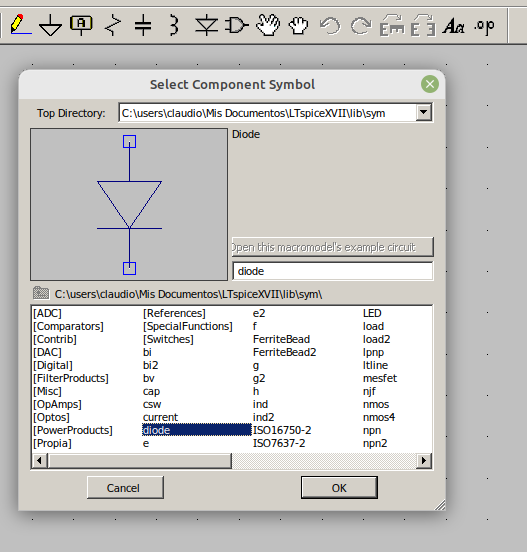
\includegraphics[width=0.5\linewidth]{figuras/xxx.png}
%    \caption{Enter Caption}
%    \label{fig:enter-labelxx}
%\end{figure}

\section{Punto de operación en continua}\label{puntoop}

\hspace{10pt} La directiva SPICE \textit{.op} calcula el punto de operación en corriente continua, es decir evalúa el circuito en regimen permanente considerando sólo las fuentes de continua. Por lo tanto considera a los capacitores como circuito abierto y los inductores como corto circuito. En la figura \ref{fig 1-1} se muestra el resultado de la directiva \emph{.op}, se ve en la ecuación \ref{eq1} que las corrientes y las tensiones de continua son las que se obtienen por simple aplicación de la teoría de los circuitos: 



\begin{equation} \label{eq1}
\begin{split}
I(R_1)=I(R_2) &= \displaystyle {\frac{10V}{2200\Omega+1000\Omega}=0.003125 A } \\
V(2) &= I(R_2)\times 2200\Omega=6.875 V
\end{split}
\end{equation}




\begin{figure}
    \centering
    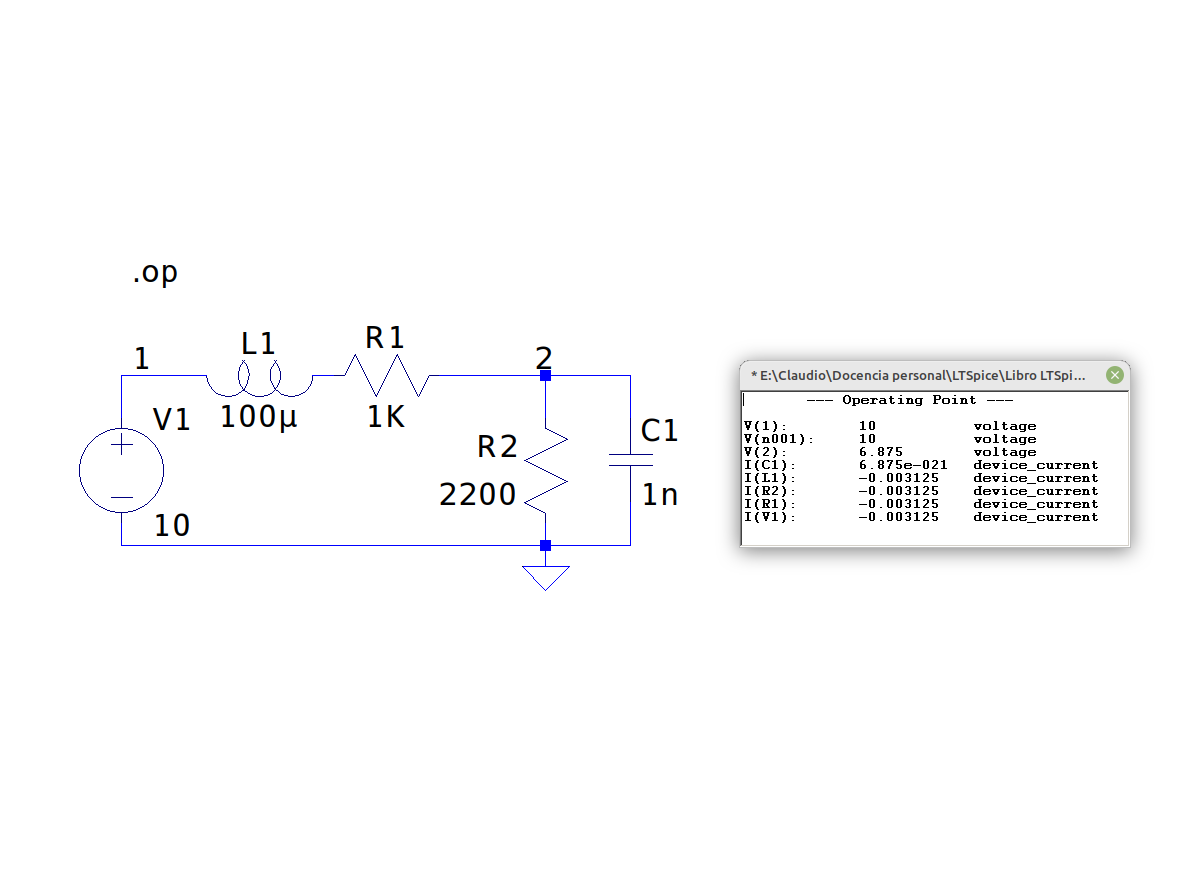
\includegraphics[width=1.0\linewidth]{figuras/fig 1-1x.png}
    \caption{Punto de operación .op}
    \label{fig 1-1}
\end{figure}

Se puede obtener también el punto de operación en continua de distintos dispositivos,  tales como diodos, transistores bipolares (TBJ), transistores MOS y JFETs. En la figura \ref{fig 1-2} se muestra un ejemplo del cálculo del punto de polarización de un TBJ de la biblioteca propia del LTSpice. De los datos obtenidos se puede calcular: $\beta = \frac{I_C(Q_1)}{I_B(Q_1)}=203.7$ y $V_{BE}=V(b)-V(e)=0.6965V$. Con estos valores, haciendo un ciruito equivalente de Thevenin entre la base y tierra, utilizando el modelo más sencillo para el cáclulo de la polarización de un TBJ y teniendo en cuenta que $V_{TH}=V_1 \frac{R_2}{R_1+R_2}=1.803V$ y $R_{TH}=\frac{R_1R_2}{R_1+R_2}=1.8033K\Omega$. Con  las ecuaciones \ref{eq2} se obtienen valores muy similares a los hallados por simulación. 

\begin{equation} \label{eq2}
\begin{split}
I_C(Q_1) &= \displaystyle{\frac{V_{TH}-V_{BE}}{\displaystyle{\frac{R_{TH}}{\beta}}+\displaystyle{\frac{\beta+1}{\beta}}R_B}}=4.81mA \\
V_{CE} &= V_1-I_C(Q_1)R_4-\frac{\beta+1}{\beta}I_C(Q_1)R_3=4.13V
\end{split}
\end{equation}




\begin{figure}
    \centering
    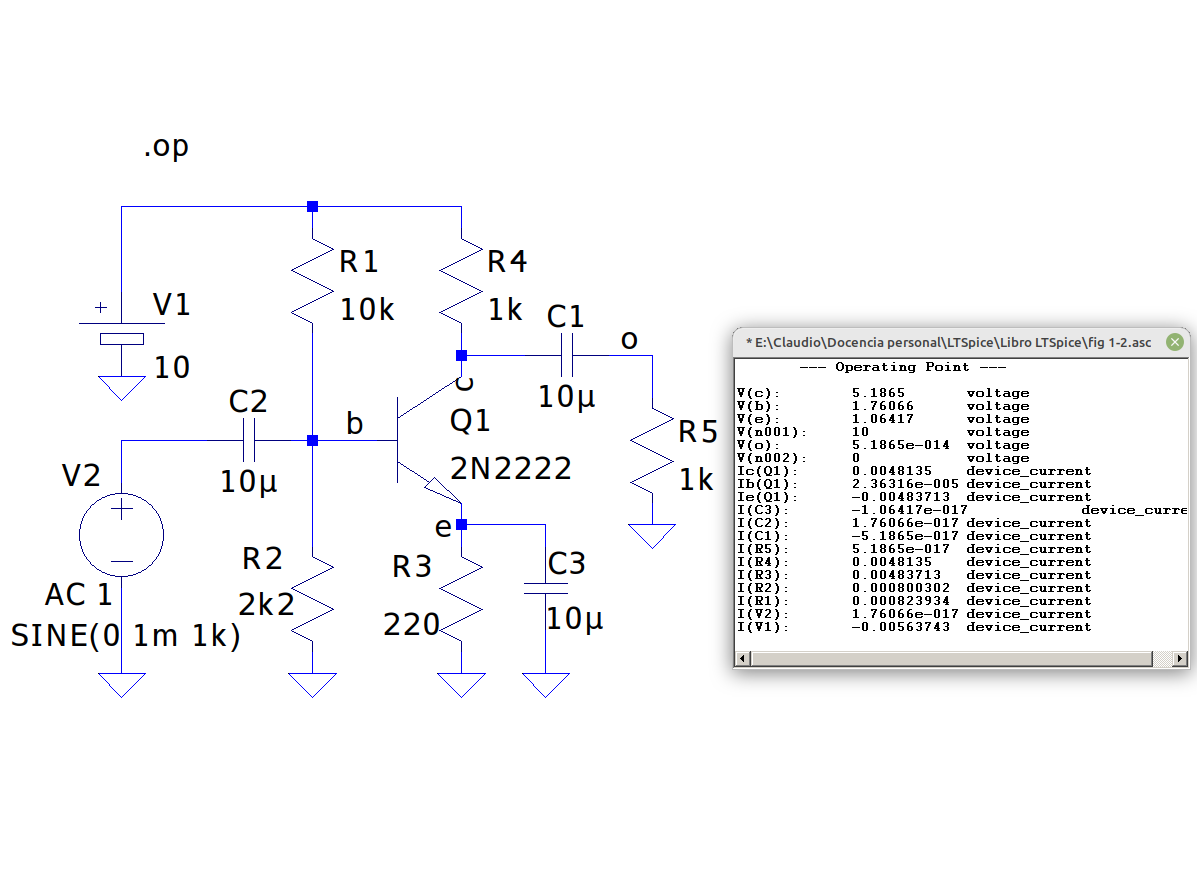
\includegraphics[width=1.0\linewidth]{figuras/fig 1-2xx.png}
    \caption{Punto de operación en un TBJ.}
    \label{fig 1-2}
\end{figure}


Cuando se ejecuta la directiva \textit{.op} se genera un archivo auxiliar en el cual se resume el punto de funcionamiento y los valores de los modelos de los dispositivos involucrados. Dicho archivo tiene una extensión \textit{.log} y se obtiene abriendo la pestaña \textit{View} y \textit{SPICE Error Log}.

En la figura \ref{fig 1-3} se muestra el texto generado. Se observan en dicho archivo las corrientes y tensiones de polarización $I_b$, $I_c$, $V_{be}$, $V_{bc}$ y $V_{ce}$; el $\beta_{DC}$ y los parámetro del modelo de  pequeña señal $g_m$, $r_{pi}$, $R_x$, $R_o$, $C_{be}$, $C_{bc}$, $C_{js}$, $C_{bx}$, $\beta_{AC}$ y $F_t$.

\begin{figure}
    \centering
    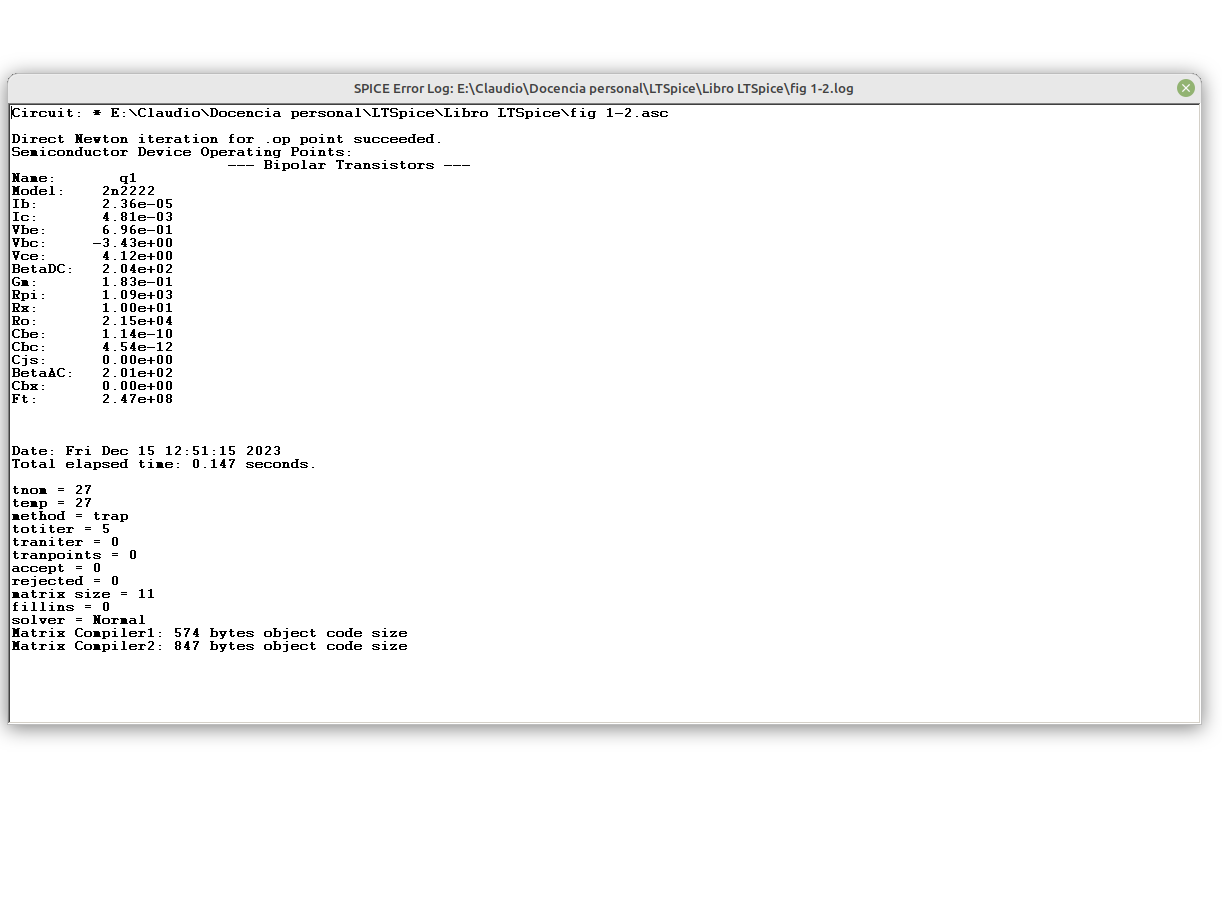
\includegraphics[width=1.0\linewidth]{figuras/fig 1-3x.png}
    \caption{Resumen del punto de operación del dispositivo.}
    \label{fig 1-3}
\end{figure}

\section{Barrido de corriente continua}

\hspace{10pt} La directiva SPICE \textit{.dc} produce un barrido de alguna fuente de tensión o corriente del circuito. 

En el circuito de la figura \ref{fig 1-4} se produce un barrido lineal de la fuente de corriente de base $I_1$ entre $10\mu A$ y $30\mu A$ en pasos de a $0.1\mu A$ (directiva SPICE \textit{.dc I1 10u 30u .1u}) , es decir se realizan 201 cálculos del punto de polarización diferentes para cada valor de la corriente $I_1$. En la ventana desplegada se ve como se indica el barrido: nombre de la fuente a barrer, tipo de barrido ( lineal, por octavas, por décadas o a partir de una lista determinada, siendo el lineal el que se toma por defecto), el valor de inicio, el de final y el paso de barrido.

Al final de la simulación se despliega una ventana de visualización, en este tipo de simulación en el eje horizontal se representa la variable que se barre ( en este caso $I_1$ ) y en el eje vertical se elije la señal a visualizar. En la figura \ref{fig 1-5} se muestran la corriente de colector $I_C(Q_1)$ y la tensión de base $V(b)$,  mediante el manejo de los cursores disponibles y suponiendo que deseamos una corriente de colector de $ \approx5mA$ , obtenemos $I_B=24.7\mu A$ y $V(b) \approx 1.8V$ que son los valores que nos permitirían diseñar las resistencias de polarización de la base para lograr la corriente de colector buscada.

\begin{figure}
    \centering
    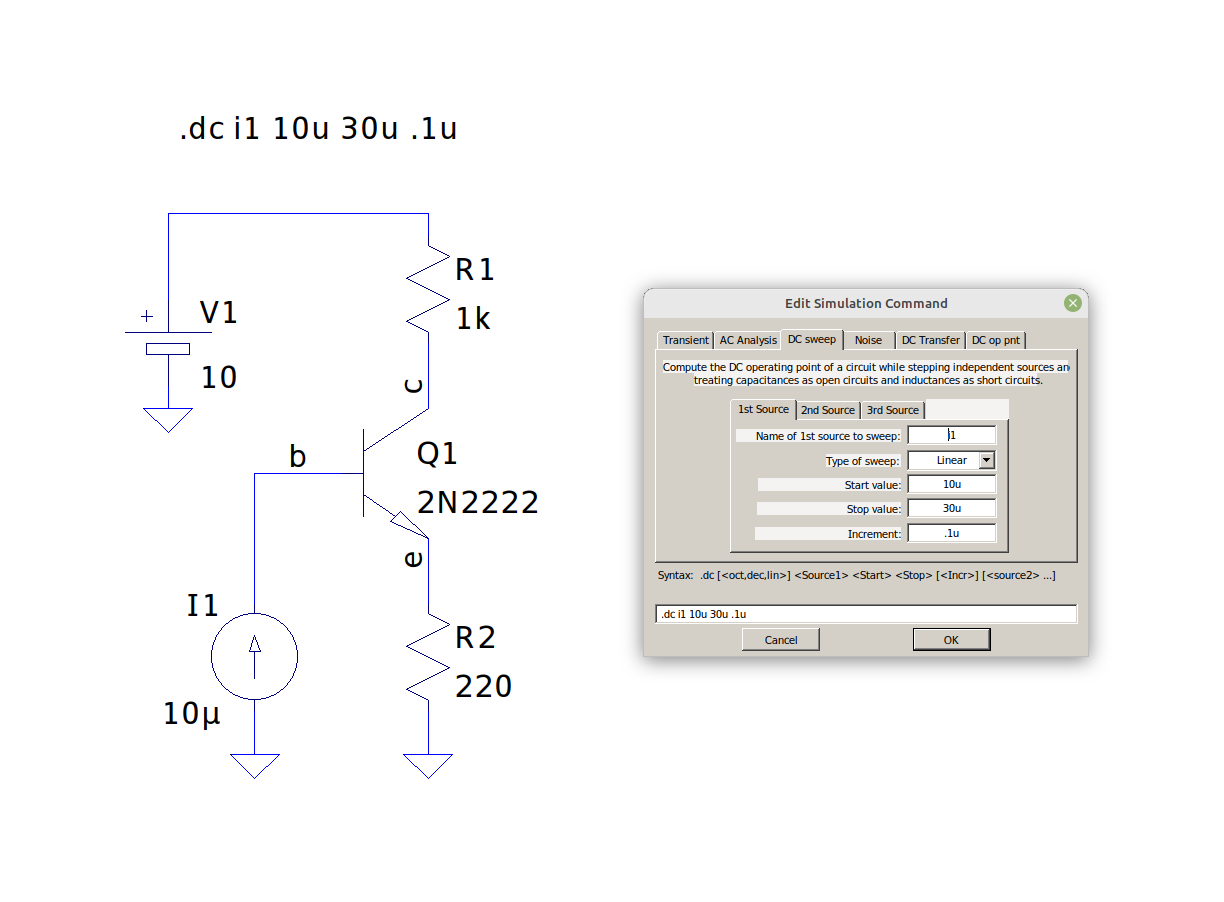
\includegraphics[width=1.0\linewidth]{figuras/fig 1-4xx.png}
    \caption{Barrido de una fuente de corriente.}
    \label{fig 1-4}
\end{figure}

\begin{figure}
    \centering
    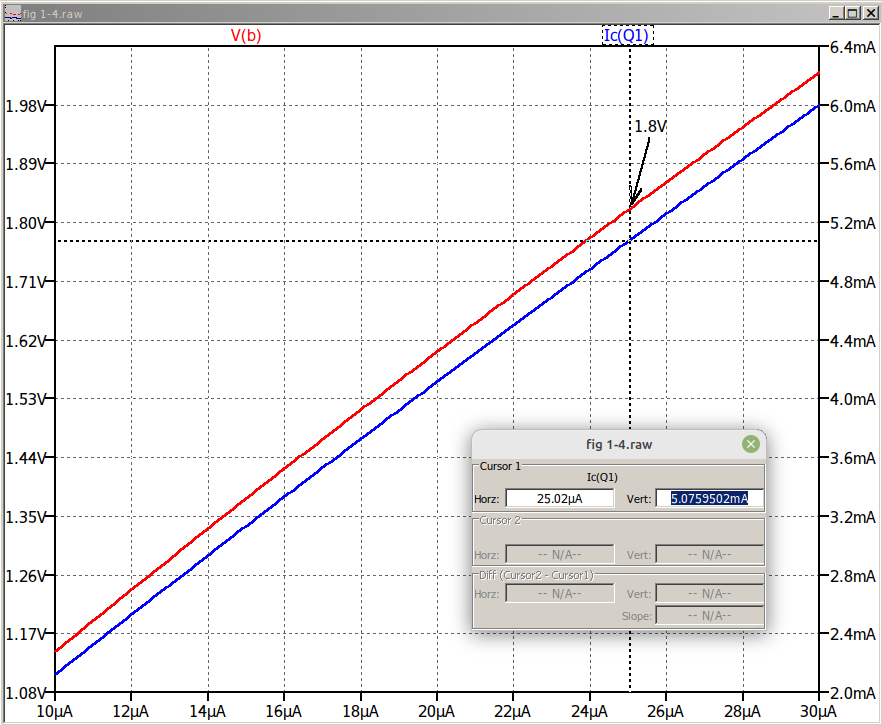
\includegraphics[width=1.0\linewidth]{figuras/fig 1-5x.png}
    \caption{Visualización del barrido de una fuente de corriente.}
    \label{fig 1-5}
\end{figure}

La directiva SPICE \textit{.dc} tiene la opción de barrido de hasta 3 fuentes de tensión o corriente diferentes en forma simultánea. Se puede utilizar esta opción para trazar las curvas de funcionamiento de algunos dispositivos. En la figura \ref{fig 1-6} se muestra el trazado de la curva de salida del TBJ 2N222, para ello se hace un barrido doble de las fuentes $V_1$ ( que es la $V_{ce}$  del TBJ) y de la fuente  $I_1$ ( la $I_B$ ) para lograr la curva paramétrica $I_C=f(V_{ce})$ con $I_B$ como parámetro, esto se logra con la directiva \textit{.dc V1 0 10 1m I1 10u 50u 10u} , que logra un barrido de la tensión $V_1$ entre 0 y 10V en pasos de 1mV para cada uno de los 5 valores de corriente $I_1$ entre 10uA y 50uA en pasos de 10uA. En la parte derecha de la figura \ref{fig 1-6} se muestra la corriente $I_C$ en función de $V_{ce}$ con $I_B$ como parámetro.

\begin{figure}
    \centering
    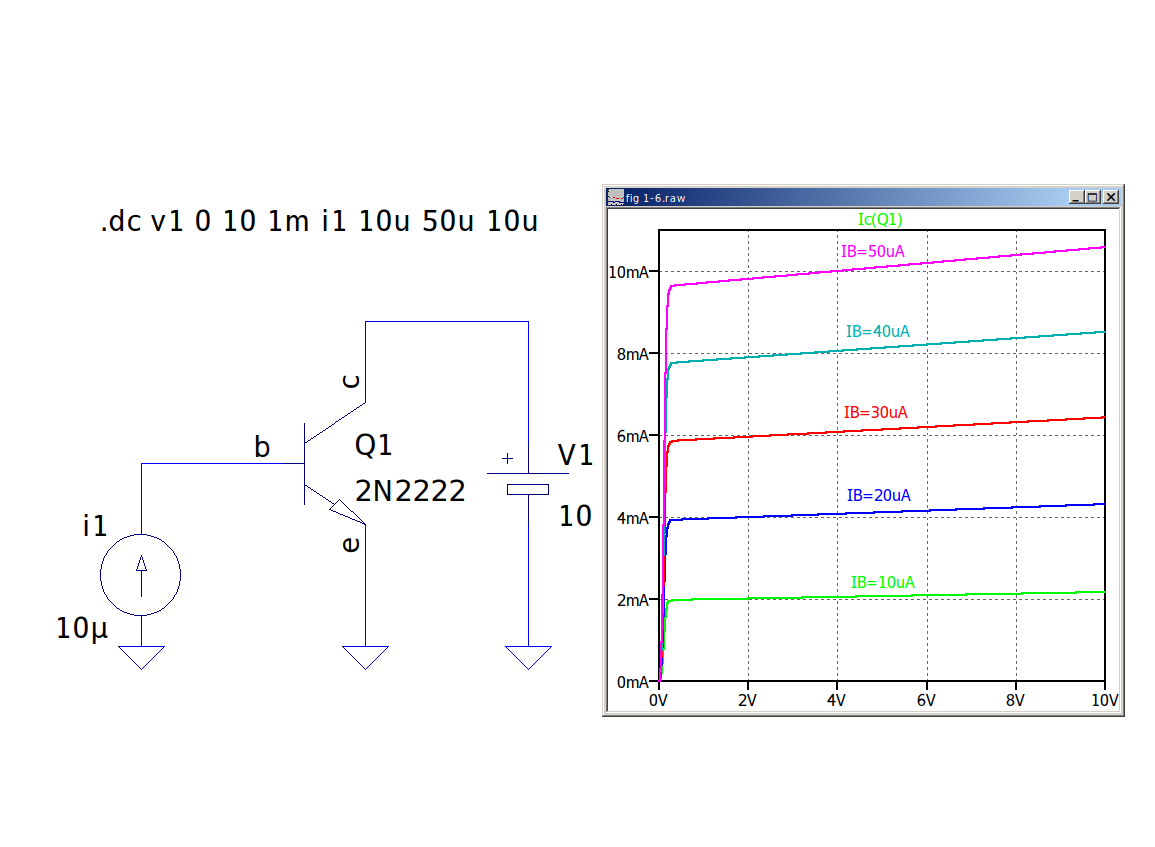
\includegraphics[width=1.0\linewidth]{figuras/fig 1-6xx.png}
    \caption{Curvas de salida del TBJ 2N222 utilizando .DC.}
    \label{fig 1-6}
\end{figure}

\section{Transferencia de continua}

\hspace{10pt} La directiva \textit{.tf} calcula la transferencia de pequeña señal en corriente continua entre una señal de salida selecionada y una fuente de tensión o corriente tomada como entrada, obtiene además la impedancia de entrada que "ve" la fuente y la impedancia de salida del circuito. En principio sólo es útil para calcular transferencias de circuitos resistivos con fuentes de corriente o tensión controladas que no dependan de la frecuencia. 

El circuito de la figura \ref{fig 1-7} es un amplificador en configuración emisor común con entrada de alterna en $V_2$ y salida $V_o$ sobre la resistencia $R_5$. Si utilizamos para el transistor bipolar el modelo de emisor común simplificado con parámetros $h_{ie}=1K\Omega$ y $h_{fe}=200$, podemos hallar la transferencia mencionada y las impedancias de entrada y salida a frecuencias medias utilizando el circuito de la fig \ref{fig 1-8}, considerarando a los capacitores externos y a la fuente de continua como corto circuito. Resolviendo el circuito por métodos tradicionales de circuitos se obtiene.



\begin{equation} \label{eq3}
\begin{split}
\frac {V_o}{V_2}&=-h_{fe}\frac{R_4||R_5}{R_{hie}}\frac{R_1||R_2||R_{hie}}{R_1||R_2||R_{hie}+R_6}=-39.1459\\
Z_i&=R_6+R_2||R_1||R_{hie}=1643.3\Omega\\
Z_o&=R_3||R_5=500\Omega
\end{split}
\end{equation}

Que es el mismo resultado que se obtiene por simulación en el circuito de la fig \ref{fig 1-8}. Se utiliza aquí una fuente de corriente controlada por corriente (F) como fuente del colector, siendo la corriente de control (la de base) la que circula por la fuente de tensión de sensado $v_x=0$, que no afecta el funcionamiento del circuito.


\begin{figure}
    \centering
    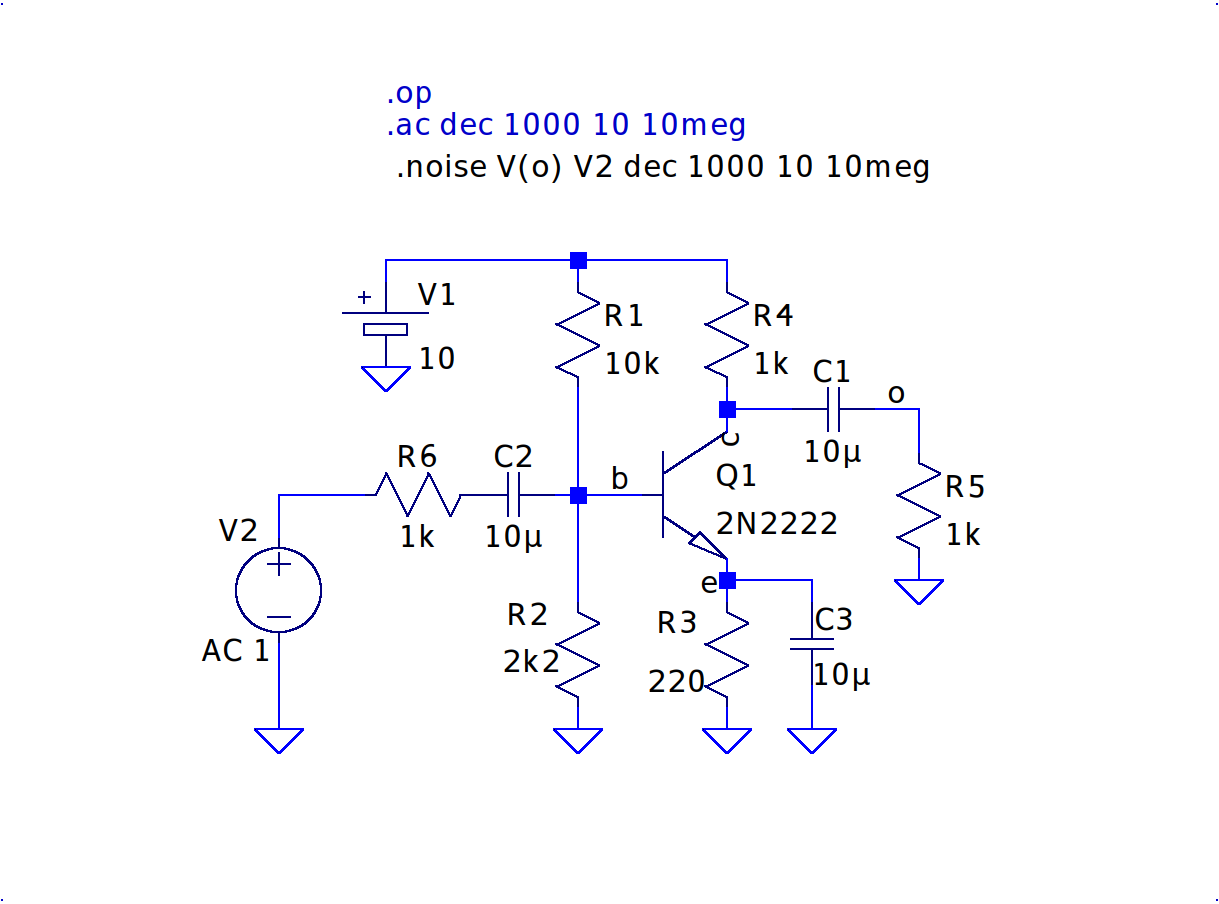
\includegraphics[width=1.0\linewidth]{figuras/fig 1-7xxx.png}
    \caption{Amplificador emisor común}
    \label{fig 1-7}
\end{figure}

\begin{figure}
    \centering
    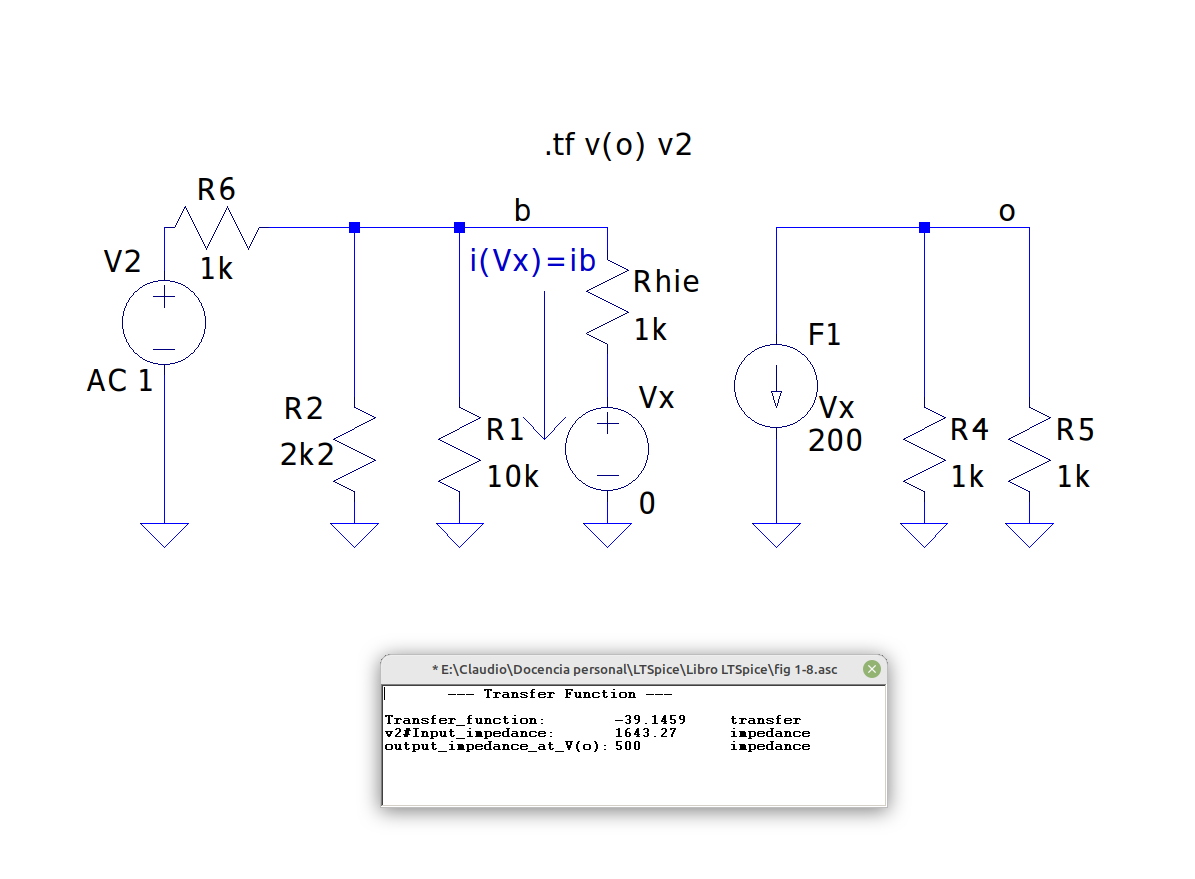
\includegraphics[width=1.0\linewidth]{figuras/fig 1-8x.png}
    \caption{Modelo de pequeña señal a frecuencias medias del amplificador emisor común.}
    \label{fig 1-8}
\end{figure}

\section{Barrido de corriente alterna}

\hspace{10pt} La directiva SPICE \textit{.ac} produce un barrido de las fuentes de corriente alterna en un rango de frecuencias determinado. Previo al análisis de alterna se realiza el cálculo del punto de operación de continua, del que se obtienen los valores de los modelos de pequeña señal de los dispositivos involucrados.  El análisis de CA es lineal y para realizarlo se utilizan los parámetros incrementales obtenidos previamente remplazando los dispositivos por sus modelos correspondientes de pequeña señal, luego de lo cual se realiza el análisis en régimem permanente de onda senoidal para cada frecuencia del barrido.

En el circuito de la fig \ref{fig 1-7} y utilizando el TBJ de biblioteca 2N222 se realiza el análisis de alterna: \textit{.ac dec 1000 10 10Meg}. La opción \textit{dec} indica que se va a hacer un tipo de barrido por décadas para obtener un diagrama de Bode de las transferencias, las siguientes opciones cuantifican el barrido: 1000 valores por década, 10 Hz la frecuencia inicial del barrido y 100 MHz la frecuencia final del barrido. Si no se elige la opción por décadas se puede optar por tipos de barrido: \textit{linear}, \textit{octave} y \textit{list}. La fuente de alterna de entrada del circuito de la fig \ref{fig 1-7} es $V_2$ y se establece de 1V por simplicidad, para que cualquier tensión del circuito visualizada sea equivalente a la transferencia referida a dicha entrada. En la fig \ref{fig 1-9} se muestra el diagrama de Bode de amplitud y fase de la transferencia de tensión entre la salida $V_o$ y la entrada $V_2$, destacándose el valor a frecuencias medias y las frecuencias superior e inferior de corte. 

\begin{figure}
    \centering
    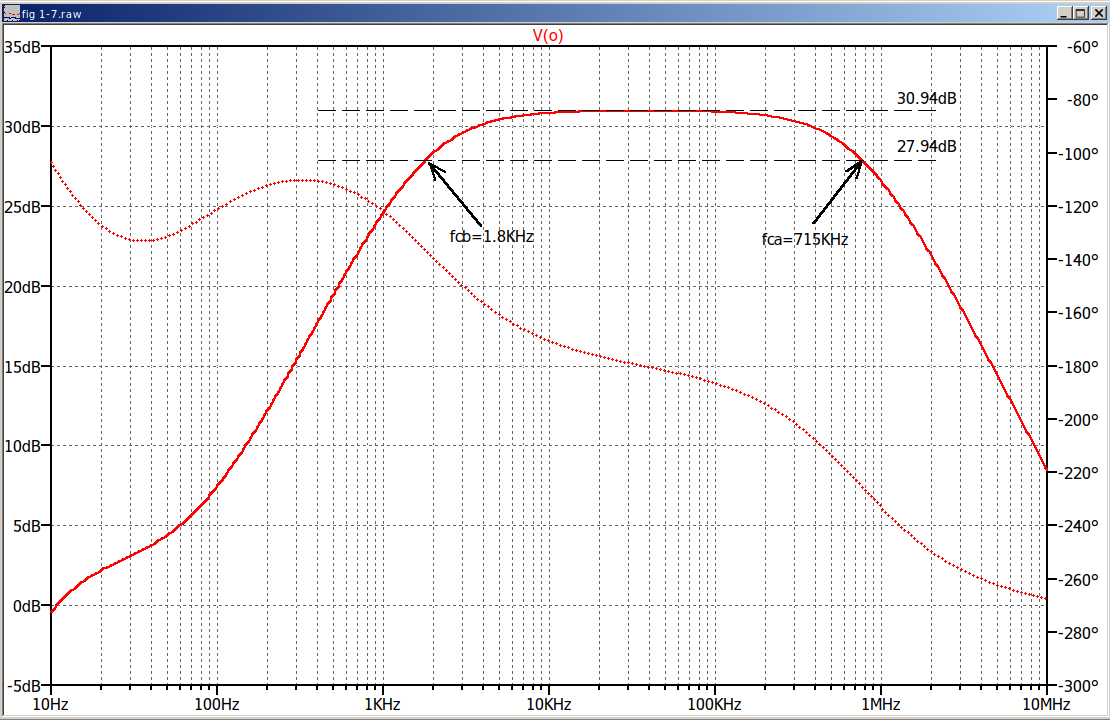
\includegraphics[width=1.0\linewidth]{figuras/fig 1-9x.png}
    \caption{Diagram de Bode de la transferencia $\frac{V_o}{V_2}$.}
    \label{fig 1-9}
\end{figure}


La directiva \emph{.noise } evalúa como el ruido generado internamente en un circuito afecta en la salida del mismo, este análisis en el dominio de la frecuencia computa el ruido tipo Johnson (térmico), el tipo shot (de emisión) y el flicker ($1/f$). Los aportes al ruido de cada componente del circuito es llevado a la fuente  no ruidosa de entrada denominada V(inoise) y la respuesta se muestra en la salida V(onoise). 

En el circuito de la fig \ref{fig 1-7} la directiva \emph{.noise V(o) V2 dec 1000 10 10meg} realiza el análisis del ruido utilizando como salida el nodo $V(o)$ y como entrada la fuente $V_2$, utilizando la opción por décadas con 1000 valores por década entre las frecuencias de 10Hz y 10MHz.

 En la fig \ref{fig 1-9-1} se grafica en la parte superior V(inoise), que es la densidad espectral del ruido referida a la entrada y  en la parte inferior V(onoise) que es la densidad espectral de ruido de la salida, ambas medidas en  $nV/\sqrt{Hz}$. Si se integra en el ancho de banda especificado la señal V(onoise), se obtiene el valor RMS del ruido a la salida, esto se logra  posicionando el mouse en la etiqueta V(onoise) y presionando  simultáneamente la tecla \emph{Ctrl} con el botón izquierdo del mouse, resultando en este caso $219,64\mu V$ como valor RMS del ruido a la salida.  
 
\begin{figure}
	\centering
	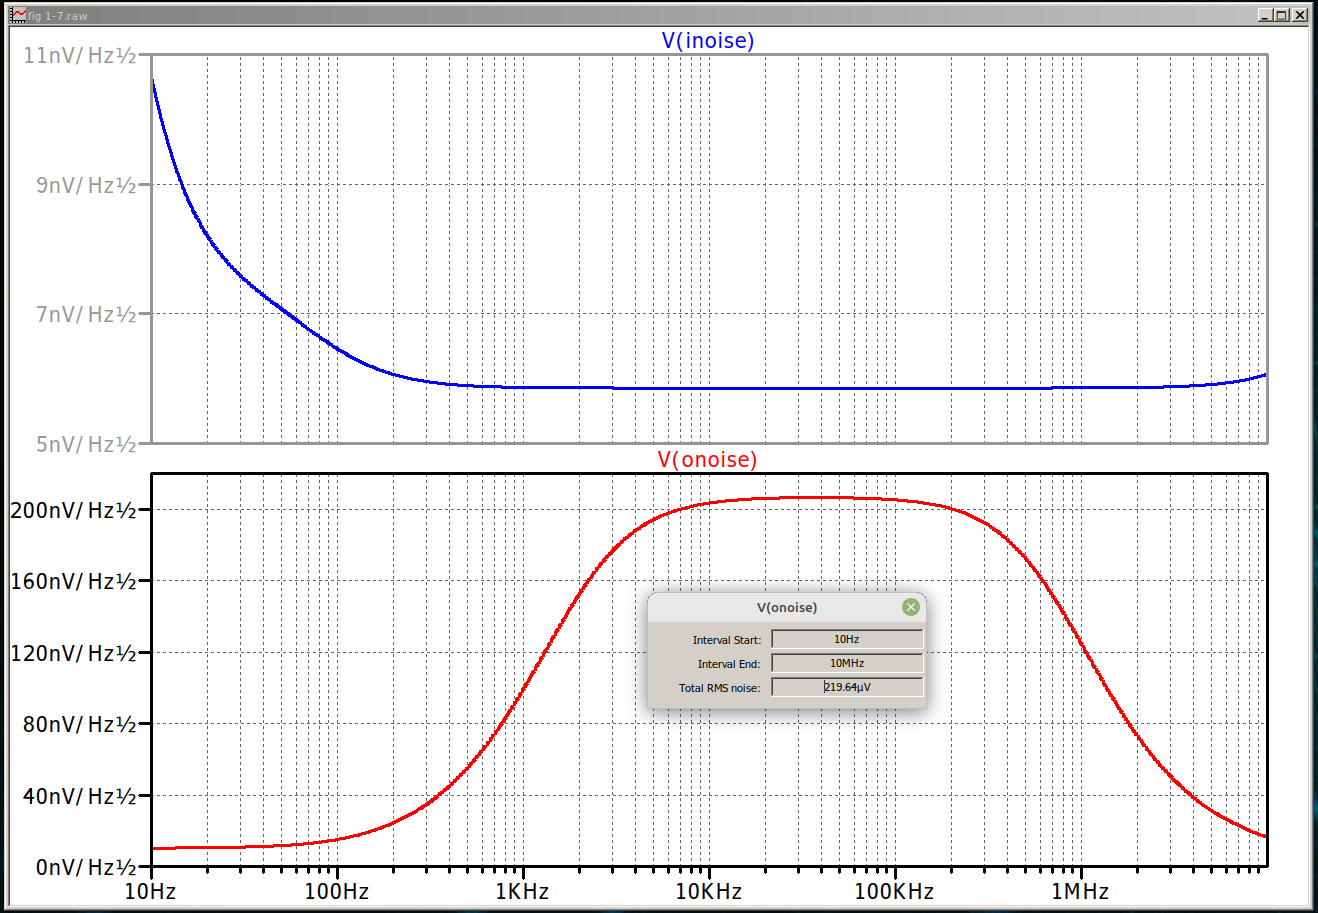
\includegraphics[width=1.0\linewidth]{figuras/fig 1-9-1.png}
	\caption{Diagram de Bode de la transferencia $\frac{V_o}{V_2}$.}
	\label{fig 1-9-1}
\end{figure}


\section{Análisis transitorio}

\hspace{10pt} La directiva SPICE \textit{.tran} realiza el análisis del circuito en el dominio del tiempo partiendo de una condición inicial determinada. En la fig \ref{fig 1-10} se muestra la simulación temporal de un rectificador de media onda, se ve la evolución transitoria de la tensión de salida $V(s)$ y la corriente por el diodo $I(D_1)$, siendo la entrada una fuente sinusoidal de 25V de pico y frecuencia 50Hz. La directiva utilizada es \textit{.tran 0 500m 0 1u} con 500ms de ventana de tiempo a simular y 1us de máximo paso de visualización.


\begin{figure}
    \centering
    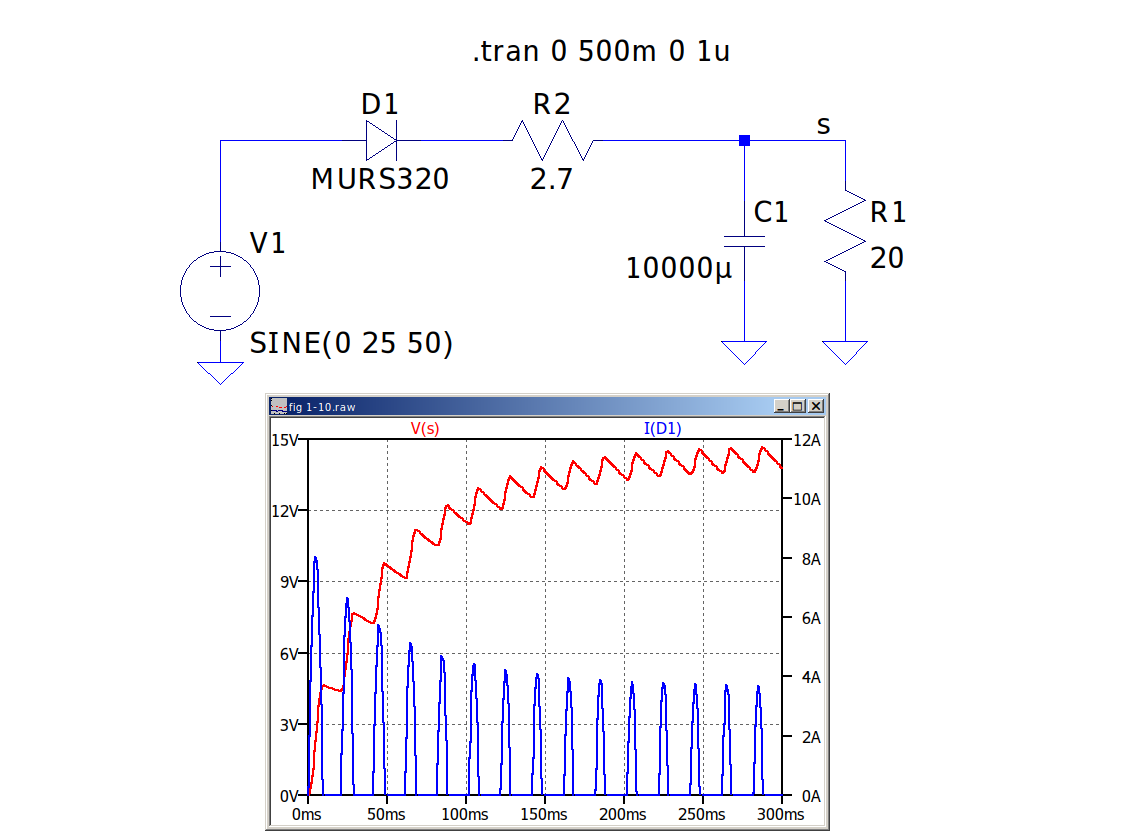
\includegraphics[width=1.0\linewidth]{figuras/fig 1-10x.png}
    \caption{Simulación temporal de un rectificador de media onda.}
    \label{fig 1-10}
\end{figure}
